\documentclass[10pt]{beamer}

\usetheme[numbering=none]{metropolis}
\usepackage{appendixnumberbeamer}

\usepackage[utf8]{inputenc}

\usepackage{booktabs}
\usepackage[scale=2]{ccicons}

\usepackage{verbatim}

\usepackage{pgfplots}
\usepgfplotslibrary{dateplot}

\usepackage{xspace}
\newcommand{\themename}{\textbf{\textsc{metropolis}}\xspace}


\title{Valaris}
\subtitle{Echtzeit Computergrafik in der Spieleentwicklung}
\date{24. Juli 2018}
\author{Frederik Lingg}
\titlegraphic{\hfill\includegraphics[height=2.5cm]{./Bilder/ValarisLogo.png}}

\begin{document}

\maketitle

\begin{frame}{Organisation}
  \begin{itemize}
    \item Aufgabenverteilung aus Entwurf beibehalten
    \item Halbwöchentliche treffen um Vortschritt/Probleme zu besprechen
    \item Weitere Kommunikation und Absprachen über Discord
    \item Festhalten des im Entwurf definierten Zeitplans in GitLab-Issues und Milestones
    \item Gruppieren von Issues durch Tags
    \item Organisation von Issues durch Boards
  \end{itemize}
\end{frame}

\begin{frame}[standout]{Tools}
    \begin{columns}[t]
        \column{.5\textwidth}
            \centering
            
\includegraphics[width=.6\textwidth]{./Bilder/intellij.png}\\
            
\includegraphics[width=\textwidth]{./Bilder/gradle.png}\\
            \vspace{.2cm}
            
\includegraphics[width=\textwidth]{./Bilder/gitlab.png}
        \column{.5\textwidth}
            \centering
            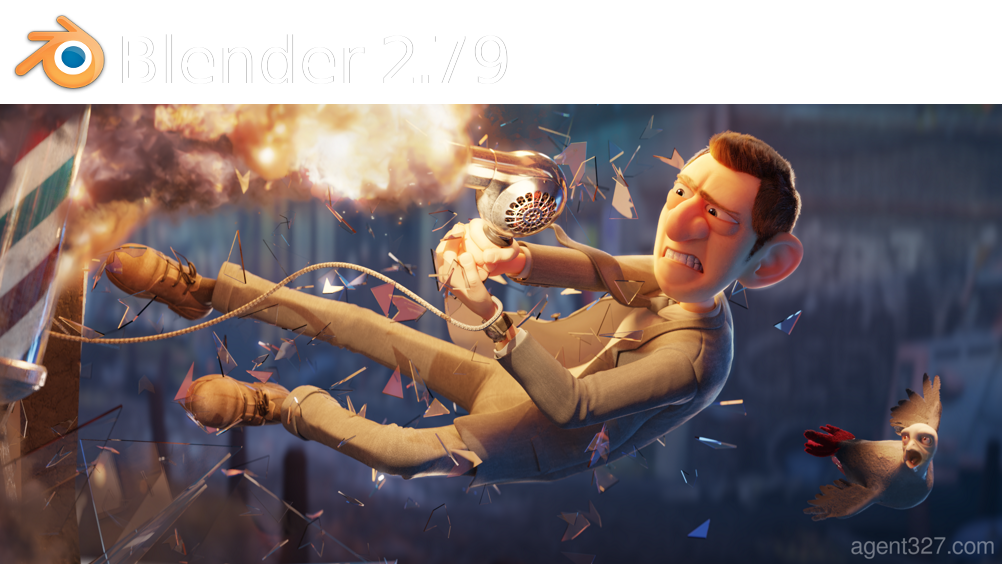
\includegraphics[width=\textwidth]{./Bilder/blender.png}\\
            \vspace{.2cm}
            
\includegraphics[width=\textwidth]{./Bilder/JmonkeyEngine.png}
    \end{columns}
\end{frame}

\begin{frame}{Features - Generierung}
\begin{itemize}
    \item Biome über Config erstellbar
    \item Tunnelassets werden verformt um dem Straßenverlauf zu folgen
    \item Dynamische Vertexreduktion und Triangulation im Dome-Terrain
\end{itemize}
\end{frame}

\begin{frame}{Features - Menu}
\begin{itemize}
    \item SplashScreen
    \item Pausemenü
    \item Hud
    \item Sprachauswahl in den Einstellungen
    \item Änderungen der Auflösung u.Ä. sind möglich ohne die Anwendung neu zu starten
\end{itemize}
\end{frame}

\begin{frame}{Features - Assets}
    \begin{itemize}
        \item Definition der AssetPacks und AssetInfos in JSON
        \item Asynchrones Laden der Assets
        \item Laden von Controls mit Reflection
        \item Automatisches klonen von Meshes wenn nötig
    \end{itemize}
\end{frame}

\begin{frame}{Features - Rendering}
\begin{itemize}
    \item Shader
    \begin{itemize}
        \item Microfacet BRDF nach UE4
        \item Image based Lighting nach UE4
        \item Pro Vertex Animation von Material-Parametern
        \item Kompatibel mit JME3-Schatten Effekten
    \end{itemize}
    \item Utility
    \begin{itemize}
        \item ViewPortManager für übersichtiliches Management der ViewPorts
        \item SceneManager für Split-Screen unterstützung und aufbauen der Szene
        \item CullingManager für simples OcclusionCulling
        \item TickProcessor zum updaten aller dynamischen Objekte in der Szene
    \end{itemize}
\end{itemize}
\end{frame}

\begin{frame}{Features - Rendering}
\begin{itemize}
    \item Partikeleffekte
    \begin{itemize}
        \item Animierte Materialien für Partikel
        \item Batching von Partikeln in einen Mesh
        \item Hinzufügen von Partikeleffekten durch hinzufügen einer Strategie möglich
    \end{itemize}
\end{itemize}
\end{frame}

\begin{frame}{Überraschende Probleme}
\begin{itemize}
    \item Rendering
    \begin{itemize}
        \item Vertex-Attribute sind Enums
        \item Gleitkomma-Zahlen sind zu ungenau (eigentlich nicht sehr überraschend)
    \end{itemize}

    \item Generierung
    \begin{itemize}
        \item Winkelberechnung in JME3 Klassen ist nicht ganz intuitiv
        \item Fehlersuche in ertser Map-Generierung sehr kompliziert -> komplett neu geschrieben
    \end{itemize}
\end{itemize}
\end{frame}

\begin{frame}{Gantt - geplant}
    \includegraphics[width=\textwidth]{./Bilder/PSE_Gantt.pdf}
\end{frame}

\begin{frame}{Gantt - tatsächlich}
    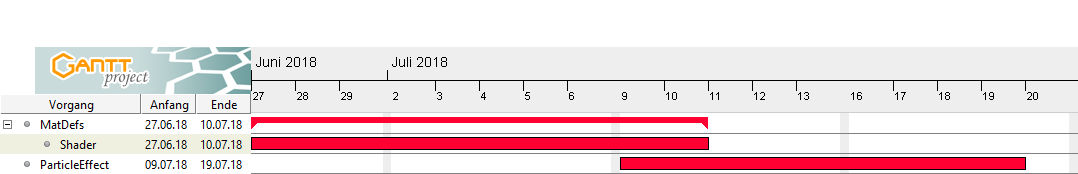
\includegraphics[width=\textwidth]{./Bilder/GanttJonas.png}\\
    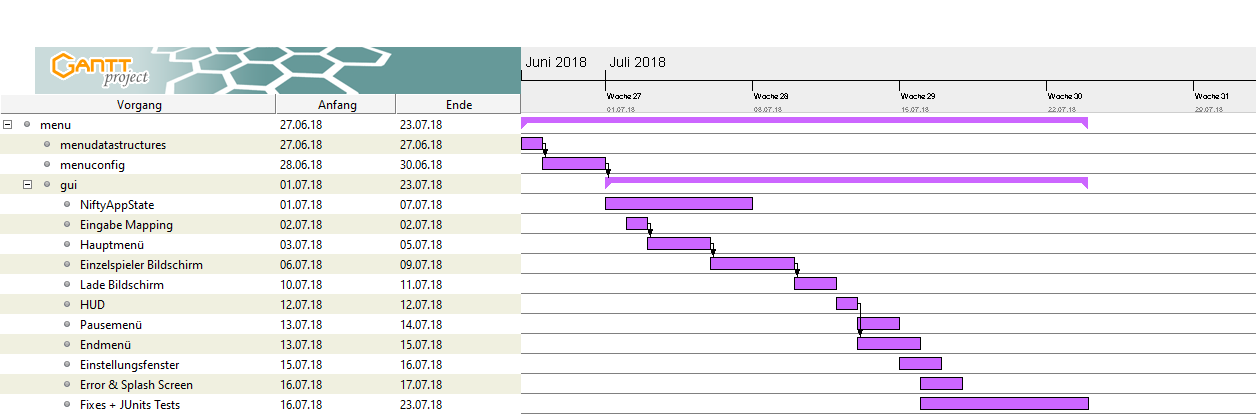
\includegraphics[width=\textwidth]{./Bilder/GanttArtur.png}\\
    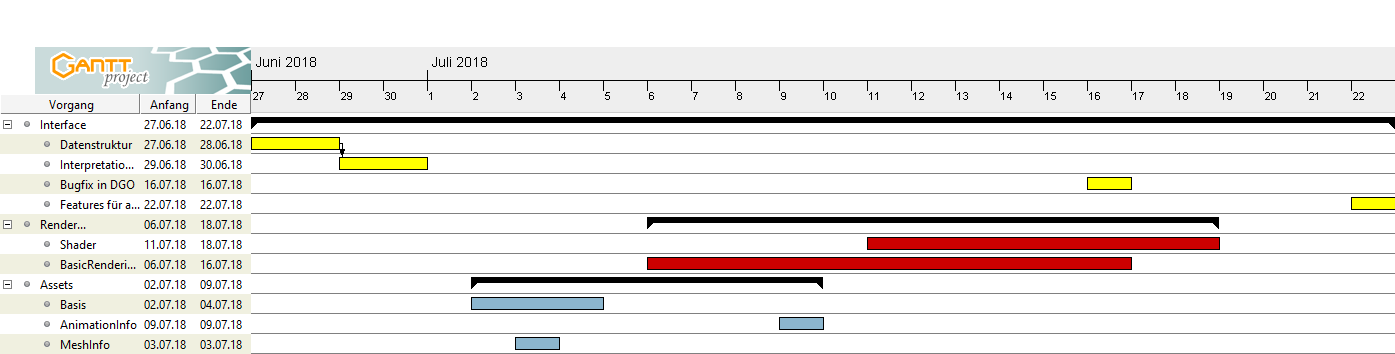
\includegraphics[width=\textwidth]{./Bilder/GanttFrederik.png}
\end{frame}

\begin{frame}{Dependencies}
\begin{itemize}
    \item Generierung
    \begin{itemize}
        \item \url{https://gist.github.com/KdotJPG/b1270127455a94ac5d19}
        \item \url{https://github.com/jdiemke/delaunay-triangulator}
    \end{itemize}
    
    \item Assets
    \begin{itemize}
        \item \url{https://github.com/FasterXML/jackson-databind}
    \end{itemize}
\end{itemize}
    
\end{frame}

\begin{frame}{Verweise}
    \begin{itemize}
        \item \url{https://www.embarc.de/wp-content/uploads/2013/10/gradle.png}
        \item \url{https://www.uni-oldenburg.de/fileadmin/_processed/d/e/csm_gitlab-logo_cba56e4a3e.png}
        \item \url{http://ubuntuhandbook.org/wp-content/uploads/2017/07/intellij-idea-ue-icon.png}
        \item \url{https://www.blender.org/wp-content/uploads/2017/08/splash_2x.png?x94355}
        \item \url{http://i.imgur.com/SRxyjR7.png}
    \end{itemize}
\end{frame}

%\appendix
\end{document}